\section{Limiter}
Instead of equalizing the signal it is possible to limit the signal instead by using a limiter. A limiter limits the signal at a certain threshold to make sure that a signal does not clip or that a membrane does not hits its coil. A limiter system is a feedforward system which can be stated as:
\begin{equation}
y(n) = g(n)\cdot x(x-D)
\end{equation}

Where an input $x(n)$ is delayed by $D$ and multiplied by a weigthing $g(n)$ to give $y(n)$ which is also seen in more detail on \autoref{fig:limiter_block}.
  

\begin{figure}[H]
\centering
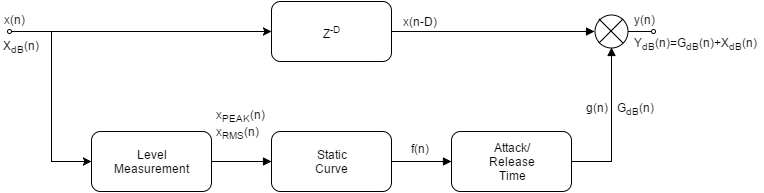
\includegraphics[width=0.8\textwidth]{figures/Limiter_block.png}
\caption{Limiter block diagram.}
\label{fig:limiter_block}
\end{figure}   

\todo[inline]{Ref til Digital Audio Signal Processing bogen kapitel syv} 

The level measurement block measures the RMS or peak value of the signal, the static curve applies the gain and the Attack/Release time determines when the limiter should apply and stop applying. The static curve more detailed described the curve which determines at which thresholds noise gate threshold (NT), expander threshold (ET), compressor threshold (CT) and limiter threshold (LT) should apply as seen on \autoref{fig:limiter_static}.

\begin{figure}[H]
\centering
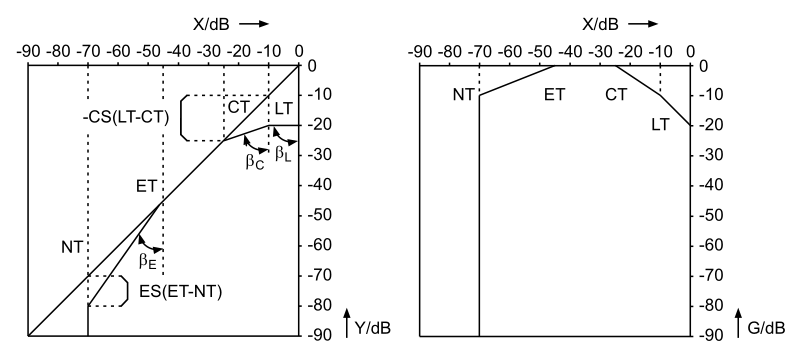
\includegraphics[width=0.8\textwidth]{figures/limiter_static_curve.png}
\caption{Static curve with the parameters (LT, CT, ET and NT).}
\label{fig:limiter_static}
\end{figure}  

Because the focus will be on limiting the signal and not clipping it, which would introduce to much distortion, the focus should be on CT which compresses the signal. A compressor decreases the change of output relative to the change in the input. The compressor can either apply to all frequencies or be a multiband compressor which only apply to the frequency spectrum which needs compression. 

      